\documentclass[12pt, titlepage]{article}

\usepackage{fullpage}
\usepackage[round]{natbib}
\usepackage{multirow}
\usepackage{booktabs}
\usepackage{tabularx}
\usepackage{graphicx}
\usepackage{float}
\usepackage{hyperref}
\usepackage{tikz}
\usetikzlibrary{positioning,arrows.meta}
\hypersetup{
    colorlinks,
    citecolor=blue,
    filecolor=black,
    linkcolor=red,
    urlcolor=blue
}

\input{../../Comments}
%% Common Parts

\newcommand{\progname}{Software Engineering} % PUT YOUR PROGRAM NAME HERE
\newcommand{\authname}{Team \#1, Sanskrit Ciphers
\\ Omar El Aref
\\ Dylan Garner
\\ Muhammad Umar Khan
\\ Aswin Kuganesan
\\ Yousef Shahin} % AUTHOR NAMES                  

\usepackage{hyperref}
    \hypersetup{colorlinks=true, linkcolor=blue, citecolor=blue, filecolor=blue,
                urlcolor=blue, unicode=false}
    \urlstyle{same}
                                


\newcounter{acnum}
\newcommand{\actheacnum}{AC\theacnum}
\newcommand{\acref}[1]{AC\ref{#1}}

\newcounter{ucnum}
\newcommand{\uctheucnum}{UC\theucnum}
\newcommand{\uref}[1]{UC\ref{#1}}

\newcounter{mnum}
\newcommand{\mthemnum}{M\themnum}
\newcommand{\mref}[1]{M\ref{#1}}

\begin{document}

\title{Module Guide for \progname{}} 
\author{\authname}
\date{\today}

\maketitle

\pagenumbering{roman}

\section{Revision History}

\begin{tabularx}{\textwidth}{p{3cm}p{2cm}X}
\toprule {\bf Date} & {\bf Version} & {\bf Notes}\\
\midrule
January 20 & 1.0 & Added sections 2-5\\
January 20 & 1.1 & Added sections 6-8\\
January 20 & 1.2 & Added sections 9-12\\
\bottomrule
\end{tabularx}

\newpage

\section{Reference Material}

This section records information for easy reference.

\subsection{Abbreviations and Acronyms}

\renewcommand{\arraystretch}{1.2}
\begin{tabular}{l l} 
  \toprule
  \textbf{symbol} & \textbf{description}\\
  \midrule
  AC & Anticipated Change\\
  AI & Artificial Intelligence\\
  API & Application Programming Interface\\
  CNN & Convolutional Neural Network\\
  CV & Computer Vision\\
  DAG & Directed Acyclic Graph \\
  JSON & JavaScript Object Notation\\
  M & Module \\
  MG & Module Guide \\
  ML & Machine Learning\\
  OCR & Optical Character Recognition\\
  OS & Operating System \\
  R & Requirement\\
  SRS & Software Requirements Specification\\
  UI & User Interface\\
  UC & Unlikely Change \\
  \bottomrule
\end{tabular}\\

\newpage

\tableofcontents

\listoftables

\listoffigures

\newpage

\pagenumbering{arabic}

\section{Introduction}

Decomposing a system into modules is a commonly accepted approach to developing
software.  A module is a work assignment for a programmer or programming
team~\citep{ParnasEtAl1984}.  We advocate a decomposition
based on the principle of information hiding~\citep{Parnas1972a}.  This
principle supports design for change, because the ``secrets'' that each module
hides represent likely future changes.  Design for change is valuable in SC,
where modifications are frequent, especially during initial development as the
solution space is explored.  

Our design follows the rules layed out by \citet{ParnasEtAl1984}, as follows:
\begin{itemize}
\item System details that are likely to change independently should be the
  secrets of separate modules.
\item Each data structure is implemented in only one module.
\item Any other program that requires information stored in a module's data
  structures must obtain it by calling access programs belonging to that module.
\end{itemize}

After completing the first stage of the design, the Software Requirements
Specification (SRS) \citep{SRS-Sanskrit-Ciphers}, the Module Guide (MG) is developed~\citep{ParnasEtAl1984}. The MG
specifies the modular structure of the system and is intended to allow both
designers and maintainers to easily identify the parts of the software.  The
potential readers of this document are as follows:

\begin{itemize}
\item New project members: This document can be a guide for a new project member
  to easily understand the overall structure and quickly find the
  relevant modules they are searching for.
\item Maintainers: The hierarchical structure of the module guide improves the
  maintainers' understanding when they need to make changes to the system. It is
  important for a maintainer to update the relevant sections of the document
  after changes have been made.
\item Designers: Once the module guide has been written, it can be used to
  check for consistency, feasibility, and flexibility. Designers can verify the
  system in various ways, such as consistency among modules, feasibility of the
  decomposition, and flexibility of the design.
\end{itemize}

The rest of the document is organized as follows. Section
\ref{SecChange} lists the anticipated and unlikely changes of the software
requirements. Section \ref{SecMH} summarizes the module decomposition that
was constructed according to the likely changes. Section \ref{SecConnection}
specifies the connections between the software requirements and the
modules. Section \ref{SecMD} gives a detailed description of the
modules. Section \ref{SecTM} includes two traceability matrices. One checks
the completeness of the design against the requirements provided in the SRS. The
other shows the relation between anticipated changes and the modules. Section
\ref{SecUse} describes the use relation between modules.

\section{Anticipated and Unlikely Changes} \label{SecChange}

This section lists possible changes to the system. According to the likeliness
of the change, the possible changes are classified into two
categories. Anticipated changes are listed in Section \ref{SecAchange}, and
unlikely changes are listed in Section \ref{SecUchange}.

\subsection{Anticipated Changes} \label{SecAchange}

Anticipated changes are the source of the information that is to be hidden
inside the modules. Ideally, changing one of the anticipated changes will only
require changing the one module that hides the associated decision. The approach
adapted here is called design for
change.

\begin{description}
\item[\refstepcounter{acnum} \actheacnum \label{acHardware}:] The specific
  hardware on which the software is running.
\item[\refstepcounter{acnum} \actheacnum \label{acInput}:] The format of the
  image input data (file formats, metadata structure).
\item[\refstepcounter{acnum} \actheacnum \label{acAuth}:] The authentication
  and authorization mechanism for different user types.
\item[\refstepcounter{acnum} \actheacnum \label{acUpload}:] The method for
  uploading and storing fragment images.
\item[\refstepcounter{acnum} \actheacnum \label{acSearch}:] The algorithm used
  for searching and filtering fragments.
\item[\refstepcounter{acnum} \actheacnum \label{acEdgeMatch}:] The machine
  learning model used for edge matching detection.
\item[\refstepcounter{acnum} \actheacnum \label{acDamage}:] The algorithm for
  fragment segmentation and feature extraction.
\item[\refstepcounter{acnum} \actheacnum \label{acScript}:] The method for
  script classification and similarity matching.
\item[\refstepcounter{acnum} \actheacnum \label{acTextSim}:] The algorithm for
  text similarity comparison.
\item[\refstepcounter{acnum} \actheacnum \label{acLineCount}:] The algorithm for
  detecting and counting text lines in fragments.
\item[\refstepcounter{acnum} \actheacnum \label{acCircleRec}:] The algorithm for
  detecting circular marks and patterns.
\item[\refstepcounter{acnum} \actheacnum \label{acEdgeClass}:] The algorithm for
  classifying edge types (torn, cut, original, burned).
\item[\refstepcounter{acnum} \actheacnum \label{acCanvas}:] The user interface
  framework for the interactive canvas.
\item[\refstepcounter{acnum} \actheacnum \label{acFragStore}:] The database
  schema and storage mechanism for fragment data.
\item[\refstepcounter{acnum} \actheacnum \label{acCatalog}:] The structure of
  catalog metadata.
\item[\refstepcounter{acnum} \actheacnum \label{acMatchOrch}:] The orchestration
  logic for combining multiple ML model results.
\item[\refstepcounter{acnum} \actheacnum \label{acSession}:] The session
  management and state persistence mechanism.
\end{description}

\subsection{Unlikely Changes} \label{SecUchange}

The module design should be as general as possible. However, a general system is
more complex. Sometimes this complexity is not necessary. Fixing some design
decisions at the system architecture stage can simplify the software design. If
these decision should later need to be changed, then many parts of the design
will potentially need to be modified. Hence, it is not intended that these
decisions will be changed.

\begin{description}
\item[\refstepcounter{ucnum} \uctheucnum \label{ucIO}:] Input/Output devices
  (Input: Image files via web upload, Output: Screen display and file export).
\item[\refstepcounter{ucnum} \uctheucnum \label{ucWebApp}:] The system will be
  deployed as a web-based application accessible through standard browsers.
\item[\refstepcounter{ucnum} \uctheucnum \label{ucImageProc}:] The system will
  process 2D images of manuscript fragments.
\item[\refstepcounter{ucnum} \uctheucnum \label{ucCollaborate}:] The system will
  support collaborative work through shared projects and annotations.
\item[\refstepcounter{ucnum} \uctheucnum \label{ucMLCore}:] Machine learning will
  be a core component for fragment matching and analysis.
\end{description}

\section{Module Hierarchy} \label{SecMH}

This section provides an overview of the module design. Modules are summarized
in a hierarchy decomposed by secrets in Table \ref{TblMH}. The modules listed
below, which are leaves in the hierarchy tree, are the modules that will
actually be implemented.

\begin{description}
\item [\refstepcounter{mnum} \mthemnum \label{mHWImageStorage}:] HW.ImageStorage Module
\item [\refstepcounter{mnum} \mthemnum \label{mCanvas}:] UI.Canvas Module
\item [\refstepcounter{mnum} \mthemnum \label{mSearch}:] UI.Search Module
\item [\refstepcounter{mnum} \mthemnum \label{mAuth}:] UI.Auth Module
\item [\refstepcounter{mnum} \mthemnum \label{mUpload}:] UI.Upload Module
\item [\refstepcounter{mnum} \mthemnum \label{mSaveSession}:] UI.SaveSession Module
\item [\refstepcounter{mnum} \mthemnum \label{mLoadSession}:] UI.LoadSession Module
\item [\refstepcounter{mnum} \mthemnum \label{mAPI}:] Svc.API Module
\item [\refstepcounter{mnum} \mthemnum \label{mSearchSvc}:] Svc.Search Module
\item [\refstepcounter{mnum} \mthemnum \label{mAuthZ}:] Svc.AuthZ Module
\item [\refstepcounter{mnum} \mthemnum \label{mSession}:] Svc.Session Module
\item [\refstepcounter{mnum} \mthemnum \label{mProcOrch}:] Svc.ProcOrch Module
\item [\refstepcounter{mnum} \mthemnum \label{mMatchOrch}:] Svc.MatchOrch Module
\item [\refstepcounter{mnum} \mthemnum \label{mFragStore}:] Data.FragmentStore Module
\item [\refstepcounter{mnum} \mthemnum \label{mCatalog}:] Data.Catalog Module
\item [\refstepcounter{mnum} \mthemnum \label{mUser}:] Data.User Module
\item [\refstepcounter{mnum} \mthemnum \label{mProject}:] Data.Project Module
\item [\refstepcounter{mnum} \mthemnum \label{mEdgeMatch}:] ML.EdgeMatch Module
\item [\refstepcounter{mnum} \mthemnum \label{mScriptClass}:] ML.ScriptClass Module
\item [\refstepcounter{mnum} \mthemnum \label{mTextSim}:] ML.TextSim Module
\item [\refstepcounter{mnum} \mthemnum \label{mSegmentation}:] ML.Segmentation Module
\item [\refstepcounter{mnum} \mthemnum \label{mCircleRecognition}:] ML.CircleRecognition Module
\item [\refstepcounter{mnum} \mthemnum \label{mLineCount}:] ML.LineCount Module
\item [\refstepcounter{mnum} \mthemnum \label{mEdgeClassification}:] ML.EdgeClassification Module
\item [\refstepcounter{mnum} \mthemnum \label{mError}:] Error Handling Module
\item [\refstepcounter{mnum} \mthemnum \label{mLogging}:] Logging Module
\item [\refstepcounter{mnum} \mthemnum \label{mConfig}:] Configuration Management Module
\item [\refstepcounter{mnum} \mthemnum \label{mTestStubs}:] Test Stubs Module
\end{description}


\begin{table}[h!]
\centering
\begin{tabular}{p{0.3\textwidth} p{0.6\textwidth}}
\toprule
\textbf{Level 1} & \textbf{Level 2}\\
\midrule

{Hardware-Hiding} & Image Storage Interface \\
\midrule

\multirow{15}{0.3\textwidth}{Behaviour-Hiding} & User Interface: UI.Canvas, UI.Search, UI.Auth, UI.Upload,\\
& \quad\quad\quad\quad\quad\quad UI.SaveSession, UI.LoadSession\\
& Service Layer: Svc.API, Svc.Search, Svc.AuthZ, Svc.Session,\\
& \quad\quad\quad\quad\quad\quad Svc.ProcOrch, Svc.MatchOrch\\
& Data Management: Data.FragmentStore, Data.Catalog,\\
& \quad\quad\quad\quad\quad\quad Data.User, Data.Project\\
& Machine Learning Modules: ML.EdgeMatch, ML.ScriptClass,\\
& \quad\quad\quad\quad\quad\quad ML.TextSim, ML.Segmentation, ML.CircleRecognition,\\
& \quad\quad\quad\quad\quad\quad ML.LineCount, ML.EdgeClassification\\
\midrule

\multirow{3}{0.3\textwidth}{Software Decision} & Utility and Support Modules (Error Handling, Logging,\\
& Configuration Management, Test Stubs)\\
\bottomrule
\end{tabular}
\end{table}
\section{Connection Between Requirements and Design} \label{SecConnection}

The design of the system is intended to satisfy the requirements developed in
the SRS. In this stage, the system is decomposed into modules. The connection
between requirements and modules is listed in Table~\ref{TblRT}. \newline

FR1.1 (User Authentication) is implemented through the \mref{mAuth} and \mref{mAuthZ} modules which manage credential verification and secure access control.
Similarly, FR1.2 (Fragment Management) and FR1.3 (Display Fragments) are supported by the \mref{mCanvas}, \mref{mUpload}, and \mref{mFragStore} modules that
enable fragment visualization and organization. Session management is enhanced by \mref{mSaveSession} and \mref{mLoadSession} modules for workspace persistence.
The ML-oriented requirements FR3.1-FR3.3 are implemented by specialized modules such as \mref{mEdgeMatch},
\mref{mScriptClass}, \mref{mSegmentation}, and \mref{mEdgeClassification}, coordinated by \mref{mMatchOrch}.

Non-functional requirements are distributed across multiple layers of the system. NFR1.1 (Usability) and NFR1.2 (Performance) are primarily addressed
by front-end and orchestration modules to ensure responsiveness and ease of interaction. NFR2.1 (Scalability) and NFR2.2 (Reliability) are achieved through
the use of modular orchestration, structured data storage, and robust error handling in modules such as \mref{mProcOrch}, \mref{mCatalog}, and \mref{mError}.
Finally, NFR3.1-NFR3.3 (Accuracy, Efficiency, and Maintainability) govern the design of the AI/ML cluster, ensuring that the models (\mref{mEdgeMatch},
\mref{mSegmentation}, \mref{mTextSim}, \mref{mLineCount}, \mref{mCircleRecognition}, \mref{mEdgeClassification}) can be retrained, tuned, and maintained without disrupting other components.

\section{Module Decomposition} \label{SecMD}

Modules are decomposed according to the principle of ``information hiding''
proposed by \citet{ParnasEtAl1984}. The \emph{Secrets} field in a module
decomposition is a brief statement of the design decision hidden by the
module. The \emph{Services} field specifies \emph{what} the module will do
without documenting \emph{how} to do it. For each module, a suggestion for the
implementing software is given under the \emph{Implemented By} title. If the
entry is \emph{OS}, this means that the module is provided by the operating
system or by standard programming language libraries.  \emph{\progname{}} means the
module will be implemented by the \progname{} software.

Only the leaf modules in the hierarchy have to be implemented. If a dash
(\emph{--}) is shown, this means that the module is not a leaf and will not have
to be implemented.

\subsection{Hardware Hiding Modules}

\begin{description}
\item[Secrets:]The data structure and algorithm used to implement the virtual
  hardware.
\item[Services:]Serves as a virtual hardware used by the rest of the
  system. This module provides the interface between the hardware and the
  software. So, the system can use it to display outputs or to accept inputs.
\item[Implemented By:] OS
\end{description}

\subsubsection{HW.ImageStorage (\mref{mHWImageStorage})}

\begin{description}
\item[Secrets:] Data structure and algorithms used to implement the image storage
\item[Services:] This module provides platform-specific file operations such as image storage and retrieval, and it serves as virtual hardware for the system.  
\item[Implemented By:] Cloud or Local Storage Interface
\item[Type of Module:] Abstract Object
\end{description}



\subsection{Behaviour-Hiding Module}

\begin{description}
\item[Secrets:]The contents of the required behaviours.
\item[Services:]Includes programs that provide externally visible behaviour of
  the system as specified in the software requirements specification (SRS)
  documents. This module serves as a communication layer between the
  hardware-hiding module and the software decision module. The programs in this
  module will need to change if there are changes in the SRS.
\item[Implemented By:] --
\end{description}

\subsubsection{UI.Canvas (\mref{mCanvas})}

\begin{description}
\item[Secrets:] The implementation of the interactive canvas for fragment manipulation.
\item[Services:] Provides an interactive interface to arrange multiple fragments and displays match suggestions
\item[Implemented By:] Front-End Web Client (React/Next.js component)
\item[Type of Module:] Abstract Object
\end{description}

\subsubsection{UI.Search (\mref{mSearch})}

\begin{description}
\item[Secrets:] The user interface design for search and filtering functionality.
\item[Services:] Provides a search interface for fragments, and supports search by script type, line count, and fragment size.
\item[Implemented By:] Front-End Web Client (React/Next.js component)
\item[Type of Module:] Abstract Object
\end{description}

\subsubsection{UI.Auth (\mref{mAuth})}

\begin{description}
\item[Secrets:] The user interface for authentication and user management.
\item[Services:] Provides login/logout interface, user registration, role-based access control UI, and session management display.
\item[Implemented By:] Front-End Authentication Component
\item[Type of Module:] Abstract Object
\end{description}

\subsubsection{UI.Upload (\mref{mUpload})}

\begin{description}
\item[Secrets:] The user interface for uploading fragment images and metadata.
\item[Services:] Provides a file upload interface to select and submit images to the backend for processing after validation.
\item[Implemented By:] Front-End Web Client (React/Next.js component)
\item[Type of Module:] Abstract Object
\end{description}

\subsubsection{UI.SaveSession (\mref{mSaveSession})}

\begin{description}
\item[Secrets:] The user interface for saving workspace state and session data.
\item[Services:] Provides a dialog interface to name and save the current workspace state, including fragment arrangements and annotations, for later retrieval.
\item[Implemented By:] Front-End Web Client (React/Next.js component)
\item[Type of Module:] Abstract Object
\end{description}

\subsubsection{UI.LoadSession (\mref{mLoadSession})}

\begin{description}
\item[Secrets:] The user interface for browsing and loading saved sessions.
\item[Services:] Provides a dialog interface to browse, select, and load previously saved workspace sessions, displaying session metadata and enabling restoration of reconstruction work.
\item[Implemented By:] Front-End Web Client (React/Next.js component)
\item[Type of Module:] Abstract Object
\end{description}

\subsubsection{Svc.API (\mref{mAPI})}

\begin{description}
\item[Secrets:] The RESTful API endpoint definitions and routing logic.
\item[Services:] Sends incoming HTTP requests from the UI to services and handles request validation
\item[Implemented By:] Backend API Gateway (FastAPI, Flask, or Node.js)
\item[Type of Module:] Abstract Object
\end{description}

\subsubsection{Svc.Search (\mref{mSearchSvc})}

\begin{description}
\item[Secrets:] The search algorithm and query optimization logic.
\item[Services:] This module performs efficient fragment searches over metadata and fragments, and it can export the results as a PDF or CSV file
\item[Implemented By:] Backend Search Service 
\item[Type of Module:] Abstract Object
\end{description}

\subsubsection{Svc.AuthZ (\mref{mAuthZ})}

\begin{description}
\item[Secrets:] The authentication and authorization implementation.
\item[Services:] This module validates user credentials and tokens, and it enforces access control for protected operations
\item[Implemented By:] Authentication \& Authorization Microservice
\item[Type of Module:] Abstract Object
\end{description}

\subsubsection{Svc.Session (\mref{mSession})}

\begin{description}
\item[Secrets:] The session state management and persistence mechanism.
\item[Services:] Manages user sessions and provides storage and retrieval of the saved user workspace
\item[Implemented By:] Backend Session Manager
\item[Type of Module:] Abstract Object
\end{description}

\subsubsection{Svc.ProcOrch (\mref{mProcOrch})}

\begin{description}
\item[Secrets:] The orchestration logic for image processing pipelines.
\item[Services:] Coordinates preprocessing workflows for images uploaded by user, and manages job queues for ML tasks
\item[Implemented By:] Workflow Orchestrator
\item[Type of Module:] Abstract Object
\end{description}

\subsubsection{Svc.MatchOrch (\mref{mMatchOrch})}

\begin{description}
\item[Secrets:] The algorithm for combining results from multiple ML models.
\item[Services:] Aggregates and sorts results from all ML models and provides confidence scores
\item[Implemented By:] Backend Orchestrator Service
\item[Type of Module:] Abstract Object
\end{description}

\subsubsection{Data.FragmentStore (\mref{mFragStore})}

\begin{description}
\item[Secrets:] The database schema and queries for fragment storage.
\item[Services:] Stores and retrieves fragment entities such as fragment IDs, associated image IDs, script labels, line counts, and status flags  
\item[Implemented By:] Data Access Layer
\item[Type of Module:] Abstract Data Type
\end{description}

\subsubsection{Data.Catalog (\mref{mCatalog})}

\begin{description}
\item[Secrets:] The catalog metadata structure and taxonomy.
\item[Services:] Stores mappings between internal fragments and external catalogue identifiers
\item[Implemented By:] Metadata Database
\item[Type of Module:] Abstract Data Type
\end{description}

\subsubsection{Data.User (\mref{mUser})}

\begin{description}
\item[Secrets:] The user data model and storage.
\item[Services:] Stores all user information such as accounts, credentials, roles and profile information for authentication and access control purposes
\item[Implemented By:] User Account Database Table
\item[Type of Module:] Record
\end{description}

\subsubsection{Data.Project (\mref{mProject})}

\begin{description}
\item[Secrets:] The project data structure for collaborative work.
\item[Services:] Manages project workspaces and collections and stores project-specific fragment groupings
\item[Implemented By:] Project Database Schema
\item[Type of Module:] Record
\end{description}

\subsubsection{ML.EdgeMatch (\mref{mEdgeMatch})}

\begin{description}
\item[Secrets:] Model details including weights and hyperparameters, segmentation mask and edge matching algorithms.
\item[Services:] Provides edge match similarity probability and computes edge features for images.
\item[Implemented By:] AI/ML Cluster (Python-based ML Service)
\item[Type of Module:] Abstract Object
\end{description}


\subsubsection{ML.ScriptClass (\mref{mScriptClass})}

\begin{description}
\item[Secrets:] Model architecture and hyperparameters, and script label and metadata.
\item[Services:] Determines the type of script based on text in the script and provides the script label with a confidence score.
\item[Implemented By:] AI/ML Cluster (Text Classification Service)
\item[Type of Module:] Abstract Object
\end{description}


\subsubsection{ML.TextSim (\mref{mTextSim})}

\begin{description}
\item[Secrets:] Vectorization and normalization methods, and algorithm used for checking similarity
\item[Services:] Converts text to embedding vector and compares similarity between text segments using transcribed text or manual annotations
\item[Implemented By:] AI/ML Cluster (Text Similarity Service)
\item[Type of Module:] Abstract Object
\end{description}


\subsubsection{ML.Segmentation (\mref{mSegmentation})}

\begin{description}
\item[Secrets:] Deep learning model weights and configuration for image segmentation.
\item[Services:] Performs image segmentation to identify and isolate individual fragment regions from manuscript images, detecting fragment boundaries and separating multiple fragments from a single scanned image.
\item[Implemented By:] AI/ML Cluster (Python-based ML Service)
\item[Type of Module:] Abstract Object
\end{description}


\subsubsection{ML.CircleRecognition (\mref{mCircleRecognition})}

\begin{description}
\item[Secrets:] Detection parameters and thresholds for circle recognition algorithms.
\item[Services:] Detects circular marks, holes, or decorative elements in manuscript fragments. These features serve as additional matching criteria when aligning fragments.
\item[Implemented By:] AI/ML Cluster (Python-based ML Service)
\item[Type of Module:] Abstract Object
\end{description}


\subsubsection{ML.LineCount (\mref{mLineCount})}

\begin{description}
\item[Secrets:] Line detection model parameters and spacing thresholds.
\item[Services:] Analyzes manuscript fragments to count the number of text lines present. Line count serves as a useful filtering and matching criterion during fragment search and reconstruction.
\item[Implemented By:] AI/ML Cluster (Python-based ML Service)
\item[Type of Module:] Abstract Object
\end{description}


\subsubsection{ML.EdgeClassification (\mref{mEdgeClassification})}

\begin{description}
\item[Secrets:] Edge classification model weights and feature extraction methods.
\item[Services:] Classifies fragment edges into categories such as torn, cut, original (manuscript boundary), or burned. Edge type classification improves matching accuracy by ensuring compatible edge pairs are compared.
\item[Implemented By:] AI/ML Cluster (Python-based ML Service)
\item[Type of Module:] Abstract Object
\end{description}

\subsection{Software Decision Module}

\begin{description}
\item[Secrets:] The design decision based on mathematical theorems, physical
  facts, or programming considerations. The secrets of this module are
  \emph{not} described in the SRS.
\item[Services:] Includes data structure and algorithms used in the system that
  do not provide direct interaction with the user.
  % Changes in these modules are more likely to be motivated by a desire to
  % improve performance than by externally imposed changes.
\item[Implemented By:] --
\end{description}

\subsubsection{Util.Error (\mref{mError})}

\begin{description}
\item[Secrets:] The error handling and exception management plan
\item[Services:] Defines standard error types and provides centralized error handling across all modules
\item[Implemented By:] Shared Backend Utility Package
\item[Type of Module:] Library
\end{description}


\subsubsection{Util.Logging (\mref{mLogging})}

\begin{description}
\item[Secrets:] The logging implementation and structure of the log format
\item[Services:] This module records system events and user actions, and it provides structured logging for information, warnings and errors.
\item[Implemented By:] Shared Logging Framework
\item[Type of Module:] Library
\end{description}


\subsubsection{Util.Config (\mref{mConfig})}

\begin{description}
\item[Secrets:] The configuration format and loading mechanism
\item[Services:] Loads configuration from files and provides read-only access to configuration values by providing the value or boolean based on key given.
\item[Implemented By:] Configuration Manager
\item[Type of Module:] Library
\end{description}

\subsubsection{Util.TestStub (\mref{mTestStubs})}

\begin{description}
\item[Secrets:] The mock implementations and mock model outputs
\item[Services:] This module provides stub implementations of services and ML components, and it simulates ML model responses
\item[Implemented By:] Test Utilities
\item[Type of Module:] Library
\end{description}

\section{Traceability Matrix} \label{SecTM}

This section shows two traceability matrices: between the modules and the
requirements and between the modules and the anticipated changes.

% the table should use mref, the requirements should be named, use something
% like fref
\begin{table}[H]
\centering
\begin{tabular}{p{0.2\textwidth} p{0.6\textwidth}}
\toprule
\textbf{Req.} & \textbf{Modules}\\
\midrule
FR1.1 & \mref{mAuth}, \mref{mAuthZ}, \mref{mSession}, \mref{mUser}\\
FR1.2 & \mref{mCanvas}, \mref{mUpload}, \mref{mAPI}, \mref{mProcOrch}, \mref{mFragStore}, \mref{mCatalog}, \mref{mSegmentation}\\
FR1.3 & \mref{mCanvas}, \mref{mSearch}, \mref{mAPI}, \mref{mLineCount}\\
FR1.4 & \mref{mCanvas}, \mref{mMatchOrch}, \mref{mEdgeMatch}, \mref{mScriptClass}, \mref{mTextSim}, \mref{mFragStore}, \mref{mCircleRecognition}, \mref{mEdgeClassification}\\
FR1.5 & \mref{mCanvas}, \mref{mAuth}, \mref{mSession}, \mref{mProject}, \mref{mSaveSession}, \mref{mLoadSession}\\
NFR1.1 & \mref{mCanvas}, \mref{mSearch}, \mref{mAuth}, \mref{mUpload}, \mref{mSaveSession}, \mref{mLoadSession}\\
NFR1.2 & \mref{mHWImageStorage}, \mref{mCanvas}, \mref{mUpload}, \mref{mAPI}\\
FR2.1 & \mref{mAPI}, \mref{mAuthZ}, \mref{mSession}, \mref{mMatchOrch}\\
FR2.2 & \mref{mAuthZ}, \mref{mSession}, \mref{mUser}\\
FR2.3 & \mref{mFragStore}, \mref{mCatalog}, \mref{mUser}, \mref{mProject}\\
NFR2.1 & \mref{mAPI}, \mref{mProcOrch}, \mref{mMatchOrch}, \mref{mHWImageStorage}\\
NFR2.2 & \mref{mFragStore}, \mref{mCatalog}, \mref{mUser}, \mref{mProject}, \mref{mError}, \mref{mLogging}, \mref{mConfig}\\
FR3.1 & \mref{mEdgeMatch}, \mref{mMatchOrch}, \mref{mEdgeClassification}\\
FR3.2 & \mref{mScriptClass}, \mref{mMatchOrch}\\
FR3.3 & \mref{mSegmentation}, \mref{mMatchOrch}, \mref{mCircleRecognition}, \mref{mLineCount}\\
NFR3.1 & \mref{mEdgeMatch}, \mref{mScriptClass}, \mref{mTextSim}, \mref{mSegmentation}, \mref{mCircleRecognition}, \mref{mLineCount}, \mref{mEdgeClassification}\\
NFR3.2 & \mref{mEdgeMatch}, \mref{mScriptClass}, \mref{mTextSim}, \mref{mSegmentation}, \mref{mCircleRecognition}, \mref{mLineCount}, \mref{mEdgeClassification}, \mref{mProcOrch}, \mref{mMatchOrch}\\
NFR3.3 & \mref{mEdgeMatch}, \mref{mScriptClass}, \mref{mTextSim}, \mref{mSegmentation}, \mref{mCircleRecognition}, \mref{mLineCount}, \mref{mEdgeClassification}, \mref{mLogging}, \mref{mConfig}, \mref{mTestStubs}\\

\bottomrule
\end{tabular}
\caption{Trace Between Requirements and Modules}
\label{TblRT}
\end{table}

\begin{table}[H]
\centering
\begin{tabular}{p{0.2\textwidth} p{0.6\textwidth}}
\toprule
\textbf{AC} & \textbf{Modules}\\
\midrule
\acref{acHardware} & \mref{mHWImageStorage}, \mref{mConfig}\\
\acref{acInput} & \mref{mUpload}, \mref{mProcOrch}, \mref{mHWImageStorage}\\
\acref{acAuth} & \mref{mAuth}, \mref{mAuthZ}, \mref{mUser}, \mref{mSession}, \mref{mAPI}\\
\acref{acUpload} & \mref{mUpload}, \mref{mProcOrch}, \mref{mFragStore}\\
\acref{acSearch} & \mref{mSearch}, \mref{mSearchSvc}, \mref{mCatalog}\\
\acref{acEdgeMatch} & \mref{mEdgeMatch}, \mref{mMatchOrch}, \mref{mEdgeClassification}\\
\acref{acDamage} & \mref{mSegmentation}, \mref{mMatchOrch}\\
\acref{acScript} & \mref{mScriptClass}, \mref{mMatchOrch}\\
\acref{acTextSim} & \mref{mTextSim}, \mref{mMatchOrch}\\
\acref{acCanvas} & \mref{mCanvas}, \mref{mSearch}, \mref{mUpload}, \mref{mSaveSession}, \mref{mLoadSession}\\
\acref{acFragStore} & \mref{mFragStore}, \mref{mCatalog}, \mref{mProject}\\
\acref{acCatalog} & \mref{mCatalog}, \mref{mSearchSvc}\\
\acref{acMatchOrch} & \mref{mMatchOrch}, \mref{mEdgeMatch}, \mref{mScriptClass}, \mref{mTextSim}, \mref{mSegmentation}, \mref{mCircleRecognition}, \mref{mLineCount}, \mref{mEdgeClassification}\\
\acref{acSession} & \mref{mSession}, \mref{mUser}, \mref{mProject}, \mref{mAuthZ}, \mref{mSaveSession}, \mref{mLoadSession}\\
\acref{acLineCount} & \mref{mLineCount}, \mref{mMatchOrch}, \mref{mSearchSvc}\\
\acref{acCircleRec} & \mref{mCircleRecognition}, \mref{mMatchOrch}\\
\acref{acEdgeClass} & \mref{mEdgeClassification}, \mref{mMatchOrch}, \mref{mEdgeMatch}\\
\bottomrule
\end{tabular}
\caption{Trace Between Anticipated Changes and Modules}
\label{TblACT}
\end{table}

\section{Use Hierarchy Between Modules} \label{SecUse}

\begin{figure}[H]
\centering
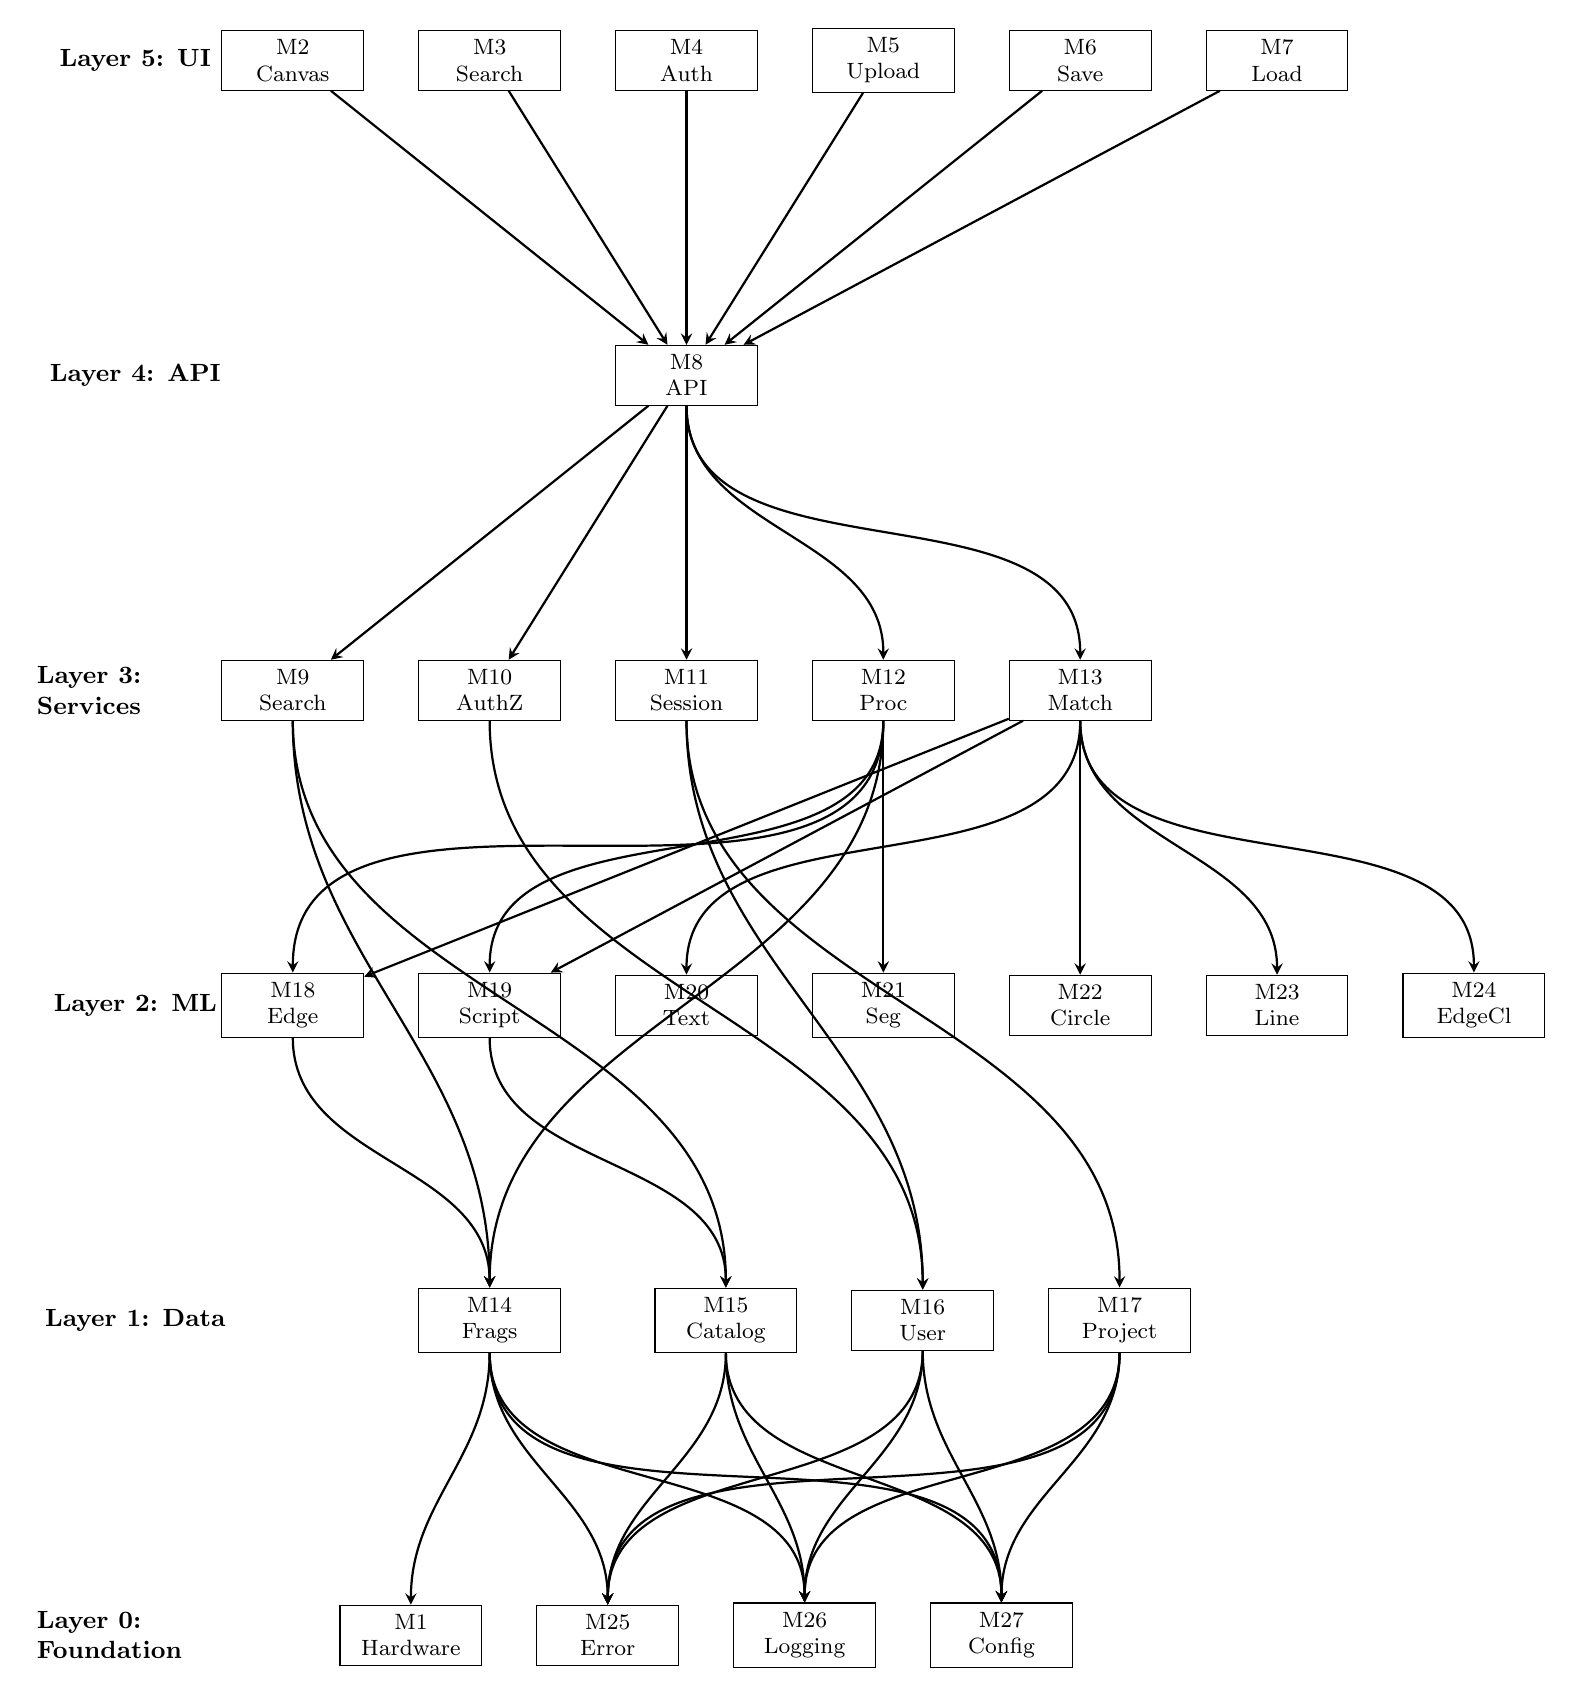
\begin{tikzpicture}[
  node distance=1.8cm and 1.2cm,
  module/.style={rectangle, draw, minimum width=1.8cm, minimum height=0.6cm, align=center, font=\footnotesize},
  direct/.style={->, >=stealth, thick},
  layer/.style={font=\bfseries\small}
]

% Layer 5 - UI
\node[layer] at (-2,10) {Layer 5: UI};
\node[module] (Canvas) at (0,10) {M2\\Canvas};
\node[module] (Search) at (2.5,10) {M3\\Search};
\node[module] (Auth) at (5,10) {M4\\Auth};
\node[module] (Upload) at (7.5,10) {M5\\Upload};
\node[module] (SaveSession) at (10,10) {M6\\Save};
\node[module] (LoadSession) at (12.5,10) {M7\\Load};

% Layer 4 - API
\node[layer] at (-2,6) {Layer 4: API};
\node[module] (API) at (5,6) {M8\\API};

% Layer 3 - Services
\node[layer, text width=2.5cm, align=left] at (-2,2) {Layer 3:\\Services};
\node[module] (SearchSvc) at (0,2) {M9\\Search};
\node[module] (AuthZ) at (2.5,2) {M10\\AuthZ};
\node[module] (Session) at (5,2) {M11\\Session};
\node[module] (ProcOrch) at (7.5,2) {M12\\Proc};
\node[module] (MatchOrch) at (10,2) {M13\\Match};

% Layer 2 - ML
\node[layer] at (-2,-2) {Layer 2: ML};
\node[module] (EdgeMatch) at (0,-2) {M18\\Edge};
\node[module] (ScriptClass) at (2.5,-2) {M19\\Script};
\node[module] (TextSim) at (5,-2) {M20\\Text};
\node[module] (Segmentation) at (7.5,-2) {M21\\Seg};
\node[module] (CircleRec) at (10,-2) {M22\\Circle};
\node[module] (LineCount) at (12.5,-2) {M23\\Line};
\node[module] (EdgeClass) at (15,-2) {M24\\EdgeCl};

% Layer 1 - Data
\node[layer] at (-2,-6) {Layer 1: Data};
\node[module] (FragStore) at (2.5,-6) {M14\\Frags};
\node[module] (Catalog) at (5.5,-6) {M15\\Catalog};
\node[module] (User) at (8,-6) {M16\\User};
\node[module] (Project) at (10.5,-6) {M17\\Project};

% Layer 0 - Foundation
\node[layer, text width=2.5cm, align=left] at (-2,-10) {Layer 0:\\Foundation};
\node[module] (HH) at (1.5,-10) {M1\\Hardware};
\node[module] (Error) at (4,-10) {M25\\Error};
\node[module] (Logging) at (6.5,-10) {M26\\Logging};
\node[module] (Config) at (9,-10) {M27\\Config};

% UI -> API (all UI modules use API)
\draw[direct] (Canvas) -- (API);
\draw[direct] (Search) -- (API);
\draw[direct] (Auth) -- (API);
\draw[direct] (Upload) -- (API);
\draw[direct] (SaveSession) -- (API);
\draw[direct] (LoadSession) -- (API);

% API -> Services (API uses all service modules)
\draw[direct] (API) -- (SearchSvc);
\draw[direct] (API) -- (AuthZ);
\draw[direct] (API) -- (Session);
\draw[direct] (API) to[out=-90, in=90] (ProcOrch);
\draw[direct] (API) to[out=-90, in=90] (MatchOrch);

% Services -> ML (orchestrators coordinate ML)
\draw[direct] (ProcOrch) to[out=-90, in=90] (EdgeMatch);
\draw[direct] (ProcOrch) to[out=-90, in=90] (ScriptClass);
\draw[direct] (ProcOrch) to[out=-90, in=90] (Segmentation);
\draw[direct] (MatchOrch) -- (EdgeMatch);
\draw[direct] (MatchOrch) -- (ScriptClass);
\draw[direct] (MatchOrch) to[out=-90, in=90] (TextSim);
\draw[direct] (MatchOrch) to[out=-90, in=90] (CircleRec);
\draw[direct] (MatchOrch) to[out=-90, in=90] (LineCount);
\draw[direct] (MatchOrch) to[out=-90, in=90] (EdgeClass);

% Services -> Data (key data access)
\draw[direct] (SearchSvc) to[out=-90, in=90] (FragStore);
\draw[direct] (SearchSvc) to[out=-90, in=90] (Catalog);
\draw[direct] (AuthZ) to[out=-90, in=90] (User);
\draw[direct] (Session) to[out=-90, in=90] (User);
\draw[direct] (Session) to[out=-90, in=90] (Project);
\draw[direct] (ProcOrch) to[out=-90, in=90] (FragStore);

% ML -> Data (ML modules use FragStore)
\draw[direct] (EdgeMatch) to[out=-90, in=90] (FragStore);
\draw[direct] (ScriptClass) to[out=-90, in=90] (Catalog);

% Data -> Foundation (all data modules use foundation)
\draw[direct] (FragStore) to[out=-90, in=90] (HH);
\draw[direct] (FragStore) to[out=-90, in=90] (Error);
\draw[direct] (FragStore) to[out=-90, in=90] (Logging);
\draw[direct] (FragStore) to[out=-90, in=90] (Config);
\draw[direct] (Catalog) to[out=-90, in=90] (Error);
\draw[direct] (Catalog) to[out=-90, in=90] (Logging);
\draw[direct] (Catalog) to[out=-90, in=90] (Config);
\draw[direct] (User) to[out=-90, in=90] (Error);
\draw[direct] (User) to[out=-90, in=90] (Logging);
\draw[direct] (User) to[out=-90, in=90] (Config);
\draw[direct] (Project) to[out=-90, in=90] (Error);
\draw[direct] (Project) to[out=-90, in=90] (Logging);
\draw[direct] (Project) to[out=-90, in=90] (Config);

\end{tikzpicture}
\caption{Use hierarchy among modules (simplified view showing key dependencies)}
\label{FigUH}
\end{figure}

\subsection{Uses Hierarchy Description}

The uses hierarchy follows a strict layered architecture where modules at each level depend only on services provided by lower levels. The diagram shows direct dependencies between modules, with arrows indicating the uses relationship.

\subsubsection{Layer 5: User Interface}
All UI modules communicate exclusively through the API layer:
\begin{itemize}
\item \textbf{Canvas (M2), Search (M3), Auth (M4), Upload (M5), SaveSession (M6), LoadSession (M7)} all directly use \textbf{API (M8)}
\item UI modules have no direct access to service, data, or ML layers, ensuring clean separation between presentation and business logic
\item \textbf{SaveSession (M6)} and \textbf{LoadSession (M7)} provide dedicated interfaces for workspace persistence and retrieval
\end{itemize}

\subsubsection{Layer 4: API Gateway}
\textbf{API (M8)} serves as the central gateway and coordinates all service layer modules:
\begin{itemize}
\item Directly uses all five service modules: \textbf{SearchSvc (M9)}, \textbf{AuthZ (M10)}, \textbf{Session (M11)}, \textbf{ProcOrch (M12)}, and \textbf{MatchOrch (M13)}
\item Provides unified RESTful interface to all backend services for the UI layer
\item Handles request routing, validation, response formatting, and rate limiting
\item Acts as the single entry point for all business logic operations
\end{itemize}

\subsubsection{Layer 3: Service Orchestration}
Service modules implement business logic and coordinate lower-level modules:

\paragraph{Data Access Services:}
\begin{itemize}
\item \textbf{SearchSvc (M9)} uses \textbf{FragmentStore (M14)} and \textbf{Catalog (M15)} to perform search and filtering operations across fragments
\item \textbf{AuthZ (M10)} uses \textbf{User (M16)} for credential verification and role-based authorization
\item \textbf{Session (M11)} uses \textbf{User (M16)} and \textbf{Project (M17)} to manage user sessions and collaborative workspace state
\end{itemize}

\paragraph{Orchestration Services:}
\begin{itemize}
\item \textbf{ProcOrch (M12)} orchestrates image processing pipelines by using:
  \begin{itemize}
  \item \textbf{FragmentStore (M14)} for accessing fragment images
  \item \textbf{EdgeMatch (M18)} for edge detection during preprocessing
  \item \textbf{ScriptClass (M19)} for initial script classification
  \item \textbf{Segmentation (M21)} for isolating individual fragments from images
  \end{itemize}
\item \textbf{MatchOrch (M13)} coordinates fragment matching by using:
  \begin{itemize}
  \item \textbf{EdgeMatch (M18)} for edge profile comparison
  \item \textbf{ScriptClass (M19)} for script similarity comparison
  \item \textbf{TextSim (M20)} for comparing extracted text between fragments
  \item \textbf{CircleRecognition (M22)} for matching circular marks and holes
  \item \textbf{LineCount (M23)} for filtering by text line count
  \item \textbf{EdgeClassification (M24)} for classifying edge types (torn, cut, original, burned)
  \end{itemize}
\end{itemize}

Note that ProcOrch focuses on preprocessing and feature extraction, while MatchOrch focuses on comparing fragments and ranking matches.

\subsubsection{Layer 2: Machine Learning}
ML modules provide specialized analysis capabilities:
\begin{itemize}
\item \textbf{EdgeMatch (M18)} uses \textbf{FragmentStore (M14)} to access fragment images for edge detection and comparison
\item \textbf{ScriptClass (M19)} uses both \textbf{Catalog (M15)} for script taxonomy metadata and \textbf{FragmentStore (M14)} for fragment images
\item \textbf{Segmentation (M21)} performs image segmentation to isolate individual fragments from scanned images
\item \textbf{CircleRecognition (M22)} detects circular marks, holes, or decorative elements for matching
\item \textbf{LineCount (M23)} counts text lines for filtering and matching criteria
\item \textbf{EdgeClassification (M24)} classifies fragment edges (torn, cut, original, burned) to improve matching accuracy
\item Other ML modules (\textbf{TextSim (M20)}) also use \textbf{FragmentStore (M14)} for data access (connections shown representatively to reduce visual complexity)
\item ML modules are always coordinated by service orchestrators (ProcOrch or MatchOrch), never invoked directly by the API
\end{itemize}

\subsubsection{Layer 1: Data Storage}
Data modules encapsulate all persistence operations and provide CRUD interfaces:
\begin{itemize}
\item \textbf{FragmentStore (M14)} uses:
  \begin{itemize}
  \item \textbf{Hardware Hiding (M1)} for file system and storage operations
  \item \textbf{Error Handling (M25)} for exception management
  \item \textbf{Logging (M26)} for audit trails of fragment operations
  \item \textbf{Config (M27)} for storage configuration parameters
  \end{itemize}
\item \textbf{Catalog (M15)} uses \textbf{Error Handling (M25)}, \textbf{Logging (M26)}, and \textbf{Config (M27)} for managing controlled vocabularies and metadata schemas
\item \textbf{User (M16)} uses \textbf{Error Handling (M25)}, \textbf{Logging (M26)}, and \textbf{Config (M27)} for user profile management and authentication data
\item \textbf{Project (M17)} uses \textbf{Error Handling (M25)}, \textbf{Logging (M26)}, and \textbf{Config (M27)} for collaborative workspace data
\end{itemize}

All data modules depend heavily on foundation modules to ensure reliable, configurable, and auditable data operations.

\subsubsection{Layer 0: Foundation}
Foundation modules provide cross-cutting system services with no dependencies on other system modules:
\begin{itemize}
\item \textbf{Hardware Hiding (M1)} abstracts operating system and file system operations, used by FragmentStore for persistent storage
\item \textbf{Error Handling (M25)} provides exception management and error reporting, used by all data modules and propagated throughout upper layers
\item \textbf{Logging (M26)} records system events, user actions, and audit trails, used extensively by data and service layers
\item \textbf{Config (M27)} manages application configuration from files and environment variables, used by all data modules and some services
\end{itemize}

\subsubsection{Key Architectural Properties}

The uses hierarchy exhibits several important design properties:

\begin{enumerate}
\item \textbf{Strict Layering:} All dependencies flow downward through the layer hierarchy. Modules only use modules in lower layers, never peers or higher layers, ensuring clear separation of concerns.

\item \textbf{API Gateway Pattern:} The API module (M8) serves as the single entry point for all UI modules, providing a unified interface to backend services and preventing direct UI-to-service coupling.

\item \textbf{Orchestration Pattern:} Complex workflows involving multiple ML modules are coordinated by dedicated orchestrator services (ProcOrch and MatchOrch), which hide the complexity of multi-model coordination from the API layer.

\item \textbf{Data Encapsulation:} All persistent data access flows through dedicated data modules (M14-M17), preventing direct database access from service or ML layers and enabling consistent data validation and access control.

\item \textbf{Foundation Ubiquity:} Utility modules (Error, Logging, Config) are used throughout the system, particularly by the data layer. The diagram shows representative uses of these modules by all data modules, though they are actually used more broadly throughout the system.

\item \textbf{DAG Structure:} The dependency graph forms a directed acyclic graph with no circular dependencies, which enables:
  \begin{itemize}
  \item Independent development and testing of each layer
  \item Incremental system integration from bottom to top
  \item Module substitution without affecting higher layers
  \item Clear understanding of system dependencies and impact analysis
  \end{itemize}

\item \textbf{Testable Subsets:} Each layer represents a testable subset of the system. Layer 0 can be tested independently, Layer 1 requires only Layer 0, and so on, supporting systematic integration testing.

\item \textbf{Separation of Concerns:} The architecture clearly separates presentation (Layer 5), API interface (Layer 4), business logic (Layer 3), specialized algorithms (Layer 2), persistence (Layer 1), and system utilities (Layer 0).
\end{enumerate}

This hierarchical organization supports maintainability, testability, and evolution of the system over time.

%\section*{References}

\section{User Interfaces}

The Sanskrit Manuscript Reconstruction Platform provides a web-based interface designed for Buddhist Studies scholars to interact with manuscript fragments. The interface is built using React with TypeScript and styled using CSS to ensure consistency and responsiveness.

\subsection{Primary Interface Components}

\subsubsection{Authentication Interface}
\begin{itemize}
    \item \textbf{Login Screen:} Secure credential entry with username and password fields
    \item \textbf{Session Management:} Token-based authentication with automatic session persistence
    \item \textbf{Error Handling:} Clear error messages for invalid credentials (``Invalid username or password'')
\end{itemize}

\subsubsection{Fragment Upload and Management}
\begin{itemize}
    \item \textbf{Upload Interface:} Drag-and-drop or file browser support for image uploads (JPG, PNG, TIFF formats, max 50 MB)
    \item \textbf{Preprocessing Visualization:} Real-time display of orientation correction with confidence scores
    \item \textbf{Fragment Browser:} Thumbnail grid view of uploaded fragments with metadata overlay
\end{itemize}

\subsubsection{Interactive Canvas Workspace}
\begin{itemize}
    \item \textbf{Drag-and-Drop Canvas:} Visual workspace for arranging and comparing fragments
    \item \textbf{Fragment Manipulation:} Rotation, zoom, and positioning controls with snap-to-edge functionality
    \item \textbf{Session Persistence:} Save and restore workspace arrangements
    \item \textbf{Response Time Target:} UI drag/drop feedback latency under 200 ms
\end{itemize}

\subsubsection{Search and Filter Interface}
\begin{itemize}
    \item \textbf{Search Bar:} Fragment ID search with autocomplete
    \item \textbf{Metadata Filters:} Multi-criteria filtering (script type, line count, fragment size)
    \item \textbf{Results Display:} Grid or list view with sortable columns
    \item \textbf{Export Options:} Download filtered results as CSV or PDF
\end{itemize}

\subsubsection{Matching Suggestions Display}
\begin{itemize}
    \item \textbf{Ranked Match List:} Top-ranked fragment matches with similarity scores and confidence levels
    \item \textbf{Visual Comparison:} Side-by-side or overlay view for comparing fragments
    \item \textbf{Trust Signals:} Confidence scores, edge pattern overlays, and match explanations
\end{itemize}

\subsubsection{Transcription Assistance}
\begin{itemize}
    \item \textbf{OCR Output Display:} Extracted text with character-level confidence indicators
    \item \textbf{Script Classification:} Display of identified script type (e.g., Gupta, Tibetan, Chinese) with confidence $\geq$ 70\%
    \item \textbf{Manual Correction:} Editable text fields for scholarly review and correction
\end{itemize}
\newpage
\begin{figure}[h!]
    \centering
    \includegraphics[width=0.9\textwidth]{images/InterfaceFlowDiagram.png}
    \caption{User Interface Flow Diagram showing the complete interaction workflow from login to fragment analysis}
    \label{fig:interface_flow}
\end{figure}

\section{Design of Communication Protocols}

The Sanskrit Manuscript Reconstruction Platform uses a client-server architecture with RESTful API communication between the frontend and backend services. This section describes the communication protocols and data exchange formats.

\subsection{API Architecture}

\subsubsection{Backend API Layer}
The backend API is implemented using Flask, FastAPI, or Django (final selection to be determined during implementation) and provides versioned RESTful endpoints for all system operations.

\textbf{API Design Principles:}
\begin{itemize}
    \item \textbf{RESTful Convention:} Resource-based URLs with standard HTTP methods (GET, POST, PUT, DELETE)
    \item \textbf{Versioning:} All endpoints include version prefix (e.g., \texttt{/api/v1/})
    \item \textbf{Status Codes:} Proper HTTP status codes (200 OK, 201 Created, 400 Bad Request, 401 Unauthorized, 403 Forbidden, 404 Not Found, 500 Internal Server Error)
    \item \textbf{JSON Format:} All request and response bodies use JSON
    \item \textbf{Schema Validation:} Request/response schemas defined using Pydantic models (backend) and TypeScript interfaces (frontend)
\end{itemize}

\subsection{Core API Endpoints}

\subsubsection{Authentication Endpoints}
\begin{itemize}
    \item \texttt{POST /api/v1/auth/login} - User authentication, returns session token
    \item \texttt{POST /api/v1/auth/logout} - Session termination
    \item \texttt{GET /api/v1/auth/verify} - Token validation
\end{itemize}

\subsubsection{Fragment Management Endpoints}
\begin{itemize}
    \item \texttt{POST /api/v1/fragments/upload} - Upload fragment image (multipart/form-data)
    \item \texttt{GET /api/v1/fragments/\{id\}} - Retrieve fragment metadata and image URL
    \item \texttt{GET /api/v1/fragments} - List/search fragments with query parameters
    \item \texttt{DELETE /api/v1/fragments/\{id\}} - Delete fragment (authorized users only)
\end{itemize}

\subsubsection{Preprocessing Endpoints}
\begin{itemize}
    \item \texttt{POST /api/v1/preprocess/orientation} - Trigger orientation correction
    \item \texttt{GET /api/v1/preprocess/status/\{job\_id\}} - Check preprocessing job status
\end{itemize}

\subsubsection{Matching and Similarity Endpoints}
\begin{itemize}
    \item \texttt{POST /api/v1/matching/suggest} - Generate match suggestions for fragment
    \item \texttt{GET /api/v1/matching/results/\{fragment\_id\}} - Retrieve ranked match list
\end{itemize}

\subsubsection{OCR and Script Identification Endpoints}
\begin{itemize}
    \item \texttt{POST /api/v1/ocr/transcribe} - Extract text from fragment image
    \item \texttt{POST /api/v1/classification/script} - Identify script type
    \item \texttt{GET /api/v1/ocr/results/\{fragment\_id\}} - Retrieve OCR output
\end{itemize}

\subsubsection{Session and Workspace Endpoints}
\begin{itemize}
    \item \texttt{POST /api/v1/sessions} - Create new canvas workspace session
    \item \texttt{PUT /api/v1/sessions/\{id\}} - Update/save workspace state
    \item \texttt{GET /api/v1/sessions/\{id\}} - Restore workspace session
    \item \texttt{DELETE /api/v1/sessions/\{id\}} - Delete session
\end{itemize}

\subsection{Data Exchange Formats}

\subsubsection{Request Schema Example (Fragment Upload)}
\begin{verbatim}
POST /api/v1/fragments/upload
Content-Type: multipart/form-data

{
    "file": <binary image data>,
    "metadata": {
        "collection": "British Library",
        "shelfmark": "BL-12345",
        "provenance": "Gandhara",
        "notes": "Optional user notes"
    }
}
\end{verbatim}

\subsubsection{Response Schema Example (Match Suggestions)}
\begin{verbatim}
GET /api/v1/matching/results/{fragment_id}
Response: 200 OK

{
    "fragment_id": "BL-12345",
    "matches": [
        {
            "match_id": "BL-67890",
            "similarity_score": 0.87,
            "confidence": 0.92,
            "match_features": ["edge_pattern", "damage_signature"],
            "thumbnail_url": "/api/v1/fragments/BL-67890/thumbnail"
        },
        ...
    ],
    "timestamp": "2025-11-11T14:30:00Z"
}
\end{verbatim}

\subsection{Inter-Service Communication}

\subsubsection{Backend to ML/AI Cluster}
The backend orchestration service communicates with AI/ML components using internal API calls or message queues:
\begin{itemize}
    \item \textbf{OCR Service:} Asynchronous job queue for text extraction
    \item \textbf{Matching Service:} Real-time or batch processing for similarity computation
    \item \textbf{Script Classification Service:} Synchronous inference requests
\end{itemize}

\subsubsection{Database Communication}
\begin{itemize}
    \item \textbf{ORM Layer:} SQLAlchemy for database abstraction (PostgreSQL or SQLite)
    \item \textbf{Query Optimization:} Indexed searches for metadata filtering
    \item \textbf{Connection Pooling:} Maintained for concurrent user support (target: 15+ concurrent users)
\end{itemize}

\subsection{Security and Data Integrity}

\begin{itemize}
    \item \textbf{Authentication:} Token-based authentication (JWT or similar)
    \item \textbf{Authorization:} Role-based access control for sensitive operations
    \item \textbf{Input Validation:} Server-side validation of all API inputs
    \item \textbf{SQL Injection Prevention:} Parameterized queries via ORM
    \item \textbf{API Rate Limiting:} Throttling to prevent abuse
    \item \textbf{HTTPS:} Encrypted communication in production deployment
\end{itemize}


\section{Timeline}

The development of the Sanskrit Manuscript Reconstruction Platform follows a phased approach, with module implementation organized by architectural layer. The timeline ensures that foundational components are established before dependent modules are developed, following the uses hierarchy described in Section \ref{SecUse}.

\subsection{Phase 1: Foundation and Infrastructure (Weeks 1-3)}

\subsubsection{Week 1: Project Setup and Foundation Modules}
\begin{itemize}
    \item \textbf{Setup Development Environment}
    \begin{itemize}
        \item Configure MongoDB, Node.js/Express backend, and React frontend repositories
        \item Set up version control, CI/CD pipelines, and development/staging environments
        \item \textit{Responsible: Full Team}
    \end{itemize}
    \item \textbf{Implement Foundation Modules (Layer 0)}
    \begin{itemize}
        \item M21: Error Handling Module - Define error types, implement centralized exception handling
        \item M22: Logging Module - Configure structured logging framework (Winston/Bunyan)
        \item M23: Configuration Management - Implement environment-based configuration loading
        \item \textit{Responsible: Yousef Shahin, Aswin Kuganesan}
    \end{itemize}
\end{itemize}

\subsubsection{Week 2-3: Data Layer Implementation}
\begin{itemize}
    \item \textbf{Hardware-Hiding Module}
    \begin{itemize}
        \item M1: Implement file storage abstraction (local/cloud storage interface)
        \item \textit{Responsible: Omar El Aref}
    \end{itemize}
    \item \textbf{Data Modules (Layer 1)}
    \begin{itemize}
        \item M14: User database schema, authentication data models
        \item M12: Fragment storage schema, image metadata, CRUD operations
        \item M13: Catalog metadata structure, controlled vocabularies
        \item M15: Project workspace schema, collaborative annotations
        \item \textit{Responsible: Umar Khan, Dylan Garner}
    \end{itemize}
\end{itemize}

\subsection{Phase 2: Service Layer and API (Weeks 4-6)}

\subsubsection{Week 4: Authentication and Session Management}
\begin{itemize}
    \item \textbf{Authentication Services (Layer 3)}
    \begin{itemize}
        \item M8: JWT-based authentication, role-based access control
        \item M9: Session state management, workspace persistence
        \item \textit{Responsible: Yousef Shahin, Aswin Kuganesan}
    \end{itemize}
    \item \textbf{API Gateway (Layer 4)}
    \begin{itemize}
        \item M6: Express.js RESTful API setup, authentication endpoints
        \item \textit{Responsible: Omar El Aref}
    \end{itemize}
\end{itemize}

\subsubsection{Week 5-6: Core Service Modules}
\begin{itemize}
    \item \textbf{Service Orchestration (Layer 3)}
    \begin{itemize}
        \item M7: Fragment search and filtering logic, query optimization
        \item M10: Image preprocessing pipeline orchestration, job queue management
        \item M11: ML model result aggregation, confidence scoring (initial implementation without ML models)
        \item \textit{Responsible: Umar Khan, Dylan Garner}
    \end{itemize}
    \item \textbf{API Endpoint Completion}
    \begin{itemize}
        \item Complete all RESTful endpoints for fragment management, search, sessions, and preprocessing
        \item \textit{Responsible: Omar El Aref, Yousef Shahin}
    \end{itemize}
\end{itemize}

\subsection{Phase 3: Machine Learning Integration (Weeks 7-10)}

\subsubsection{Week 7-8: ML Infrastructure and Basic Models}
\begin{itemize}
    \item \textbf{ML Service Setup}
    \begin{itemize}
        \item Python ML service infrastructure, REST API for ML models
        \item Model serving framework (Flask/FastAPI for Python services)
        \item \textit{Responsible: Aswin Kuganesan, Umar Khan}
    \end{itemize}
    \item \textbf{Initial ML Modules (Layer 2)}
    \begin{itemize}
        \item M16: Edge detection and matching algorithm implementation
        \item M18: Script classification model training and deployment
        \item \textit{Responsible: Dylan Garner, Yousef Shahin}
    \end{itemize}
\end{itemize}

\subsubsection{Week 9-10: Advanced ML Models}
\begin{itemize}
    \item \textbf{ML Module Completion (Layer 2)}
    \begin{itemize}
        \item M17: Damage pattern analysis and similarity scoring
        \item M19: OCR model integration (using existing libraries like Tesseract/EasyOCR, fine-tuned for ancient scripts)
        \item M20: Text similarity comparison using embeddings
        \item \textit{Responsible: Omar El Aref, Aswin Kuganesan}
    \end{itemize}
    \item \textbf{Orchestrator Integration}
    \begin{itemize}
        \item Connect ML modules to M10 and M11
        \item Implement weighted scoring and confidence calculation
        \item \textit{Responsible: Umar Khan, Dylan Garner}
    \end{itemize}
\end{itemize}

\subsection{Phase 4: User Interface Development (Weeks 8-11)}

\textit{Note: UI development runs partially in parallel with ML integration}

\subsubsection{Week 8-9: Core UI Components}
\begin{itemize}
    \item \textbf{Authentication UI (Layer 5)}
    \begin{itemize}
        \item M4: Login/logout interface, user registration, session display
        \item \textit{Responsible: Yousef Shahin}
    \end{itemize}
    \item \textbf{Fragment Management UI}
    \begin{itemize}
        \item M5: File upload interface with drag-and-drop, metadata forms
        \item M3: Search bar, filtering interface, results display
        \item \textit{Responsible: Omar El Aref, Aswin Kuganesan}
    \end{itemize}
\end{itemize}

\subsubsection{Week 10-11: Interactive Canvas}
\begin{itemize}
    \item \textbf{Canvas Workspace (Layer 5)}
    \begin{itemize}
        \item M2: Drag-and-drop canvas for fragment arrangement
        \item Real-time match visualization, collaborative workspace features
        \item Integration with M11 for displaying suggestions
        \item \textit{Responsible: Umar Khan, Dylan Garner}
    \end{itemize}
\end{itemize}

\subsection{Phase 5: Testing and Refinement (Weeks 12-14)}

\subsubsection{Week 12: Integration Testing}
\begin{itemize}
    \item \textbf{Test Infrastructure}
    \begin{itemize}
        \item Mock implementations for all services and ML components
        \item \textit{Responsible: Full Team}
    \end{itemize}
    \item \textbf{Layer-by-Layer Integration Testing}
    \begin{itemize}
        \item Test data layer with foundation modules
        \item Test service layer with data layer
        \item Test ML integration with orchestrators
        \item Test UI with complete backend
        \item \textit{Responsible: Full Team}
    \end{itemize}
\end{itemize}

\subsubsection{Week 13: Performance Optimization and ML Tuning}
\begin{itemize}
    \item Database query optimization, API response time tuning
    \item ML model fine-tuning based on test fragment dataset
    \item Concurrent user testing (target: 15+ users)
    \item \textit{Responsible: Yousef Shahin, Aswin Kuganesan, Omar El Aref}
\end{itemize}

\subsubsection{Week 14: User Acceptance Testing and Documentation}
\begin{itemize}
    \item User testing with domain experts (Buddhist Studies scholars)
    \item Bug fixes and usability improvements
    \item Complete API documentation
    \item User manual and deployment documentation
    \item \textit{Responsible: Full Team}
\end{itemize}

\subsection{Phase 6: Deployment and Monitoring (Week 15)}

\begin{itemize}
    \item Production environment setup and deployment
    \item Monitoring and logging infrastructure configuration
    \item Performance monitoring and error tracking setup
    \item Handoff and training for stakeholders
    \item \textit{Responsible: Full Team}
\end{itemize}

\textbf{Note:} For detailed task assignments, sprint planning, and issue tracking, refer to the project's GitHub repository at: \texttt{https://github.com/DylanG5/sanskrit-cipher}

\bibliographystyle {plainnat}
\bibliography{../../../refs/References}

\newpage{}

\end{document}